\chapter{Introduction}

\section{Overview of course}

Knowing just a little bit of computer science can get you started right away in actual applications. One of the goals of this course is to learn about the fascinating subject of computer science. Another is to develop algorithmic thinking skills that will help with day-to-day critical problem-solving skills. But perhaps the most important goal of the course is to develop coding skills, which will not only open up new job opportunities but also make you more effective in most areas of business. 

In the first semester, we will spend the first two classes of each week on computer science theory and special topics. The final day of each week will be a lab day, where we actually start practicing coding skills. 

In the second semester, we will start focusing more on practical coding, with a single day a week for theory and 2 lab periods per week for coding. 

Broadly, we will cover the following topics:
\begin{itemize}
    \item How modern computers work
    	\begin{itemize}
       		\item Hardware
       		\item Software
       		\item Computer networks and information systems
    	\end{itemize}
    \item Algorithms for quickly solving complex problems
    	\begin{itemize}
       		\item Searching
       		\item Sorting
    	\end{itemize}
    \item Data structures 
    	\begin{itemize}
       		\item Arrays
       		\item ArrayLists
    	\end{itemize}
    \item Applications of Computer science
    	\begin{itemize}
       		\item Basic coding in Java
       		\item How to use productivity software
    	\end{itemize}
\end{itemize}

\section{Brief history of computer science}

Timeline (credit: https://www.worldsciencefestival.com/infographics/a\_history\_of\_computer\_science/):
\begin{itemize}
\item Invention of the abacus (2700-2300 BC, Sumerians)
\item Design of first modern-style computer (Charles Babbage, 1837)
\item Design of first computer algorithm (Ada Lovelace, 1843)
\item Invention of first electronic digital computer (Konrad Zuse, 1941)
\item Invention of the transistor (Bell labs, 1947)
\item Invention of the first computer network (early Internet) (DARPA, 1968)
\item Invention of the World Wide Web (Sir Tim Berners-Lee, 1990)
\end{itemize}

\begin{figure}
	\centering
	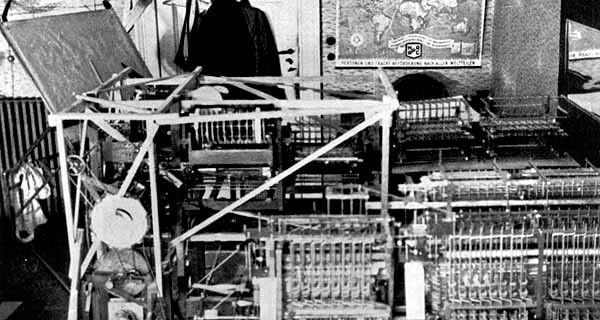
\includegraphics[width=0.85\textwidth]{images/z1.jpg}
	\caption{Construction of Konrad Zuse's Z1, the first modern computer, in his parents' apartment. Credit: https://history-computer.com/ModernComputer/Relays/Zuse.html}
	\label{fig:z1}
\end{figure}

\section{Components of a computer}

A computer is an electronic device used to process data. Its basic role is to convert data into information that is useful to people.

There are 4 primary components of a computer:

\begin{itemize}
	\item Hardware
	\item Software
	\item Data
	\item User
\end{itemize}

\subsection{Hardware}

Computer hardware consists of physical, electronic devices. These are the parts you actually can see and touch. Some examples include

\begin{itemize}
	\item Central processing unit (CPU)
	\item Monitor
	\item CD drive
	\item Keyboard
	\item Computer data storage
	\item Graphic card
	\item Sound card
	\item Speakers
	\item Motherboard
\end{itemize}

\begin{figure}
	\centering
	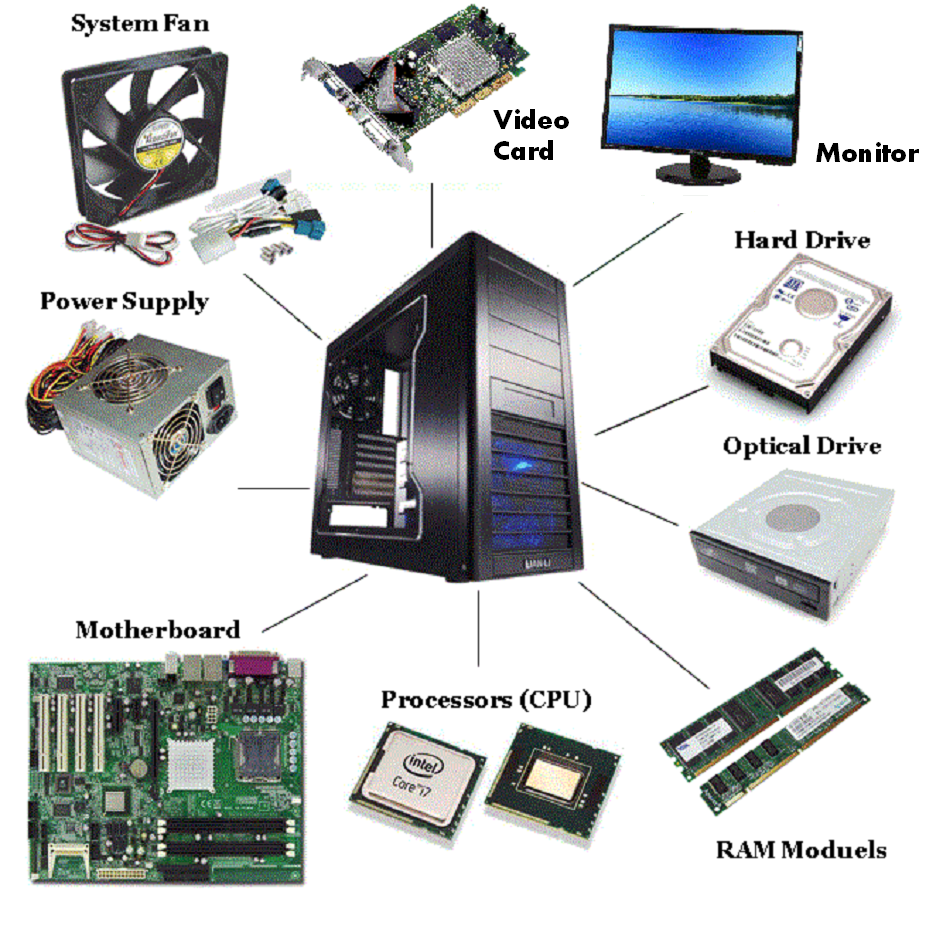
\includegraphics[width=0.85\textwidth]{images/hardware.png}
	\caption{Examples of hardware components of a personal computer. Credit: https://www5.cob.ilstu.edu/dsmath1/tag/computer-hardware/}
	\label{fig:hardware}
\end{figure}

We will discuss these components in more detail in lecture 3.

\subsection{Software}

Software (otherwise known as "programs" or "applications") are organized sets of instructions for controlling the computer.

There are two main classes of software:

\begin{itemize}
	\item Applications software: programs allowing the human to interact directly with the computer
	\item Systems software: programs the computer uses to control itself
\end{itemize}

Some more familiar applications software include

\begin{itemize}
	\item Microsoft Word: allows the user to edit text files
	\item Internet Explorer: connects the user to the world wide web
	\item iTunes: organizes and plays music files
\end{itemize}

While applications software allows the user to interact with the computer, systems software keeps the computer running. The operating system (OS) is the most common example of systems software, and it schedules tasks and manages storage of data.

We will dive deeper into the details of both applications and systems software in lecture 4.

\subsection{Data}
Data is fundamentally information of any kind. One key benefit of computers is their ability to reliably store massive quantities of data for a long time. Another is the speed with which they can do calculations on data once they receive instructions from a human user.

While humans can understand data with a wide variety of perceptions (taste, smell, hearing, touch, sight), computers read and write everything internally as "bits", or 0s and 1s.

Computers have software and hardware which allow them to convert their internal 0s and 1s into text, numerals, and images displayed on the monitor; and sounds which can be played through the speaker.

Similarly, humans have hardware and software used for converting human signals into computer-readable signals: a microphone converts sound, a camera converts pictures, and a text editor converts character symbols.

\subsection{Users}
Of course, there would be no data and no meaningful calculations without the human user. Computers are ultimately tools for making humans more powerful.

As we will see in the next section, however, different types of computers have different roles for the user.


\section{Types of computers}

\subsection{Supercomputers}
These are the most powerful computers out there. The are used for problems that take along time to calculate. They are rare because of their size and expense, and therefore primarily used by big organizations like universities, corporations, and the government.

The user of a supercomputer typically gives the computer a list of instructions, and allows the supercomputer to run on its own over the course of hours or days to complete its task.

\begin{figure}
	\centering
	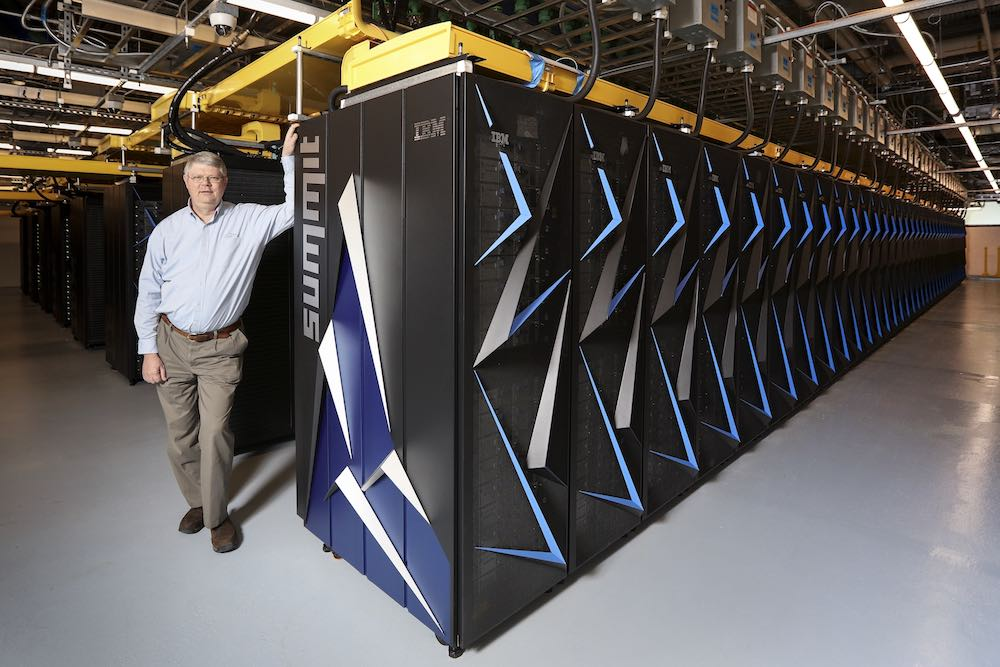
\includegraphics[width=0.85\textwidth]{images/supercomputer.jpg}
	\caption{Summit, a world-class supercomputing cluster at Oak Ridge National Laboratory in Tennessee. Credit: https://insidehpc.com/2018/11/new-top500-list-lead-doe-supercomputers/}
	\label{fig:supercomputer}
\end{figure}

\subsection{Mainframe computers}
Although not as powerful as supercomputers, mainframe computers can handle more data and run much faster than a typical personal computer. Often, they are given instructions only periodically by computer programmers, and then run on their own for months at a time to store and process incoming data. For example, census number-crunching, consumer statistics, and transactions processing all use mainframe computers

\subsection{Personal computers}
These are the familiar computers we use to interact with applications every day. Full-size desktop computers and laptop computers are examples

\subsection{Embedded computers}
In the modern "digital" age, nearly all devices we use have computers embedded within them. From cars to washing machines to watches to heating systems, most everyday appliances have a computer within them that allows them to function.

\subsection{Mobile computers}
In the past 2 decades, mobile devices have exploded onto the scene, and smartphones have essentially become as capable as standalone personal computers for many tasks.

\section{Why computers are useful}

Computers help us in most tasks in the modern age. We can use them, for example, to

\begin{itemize}
	\item write a letter
	\item do our taxes
	\item play video games
	\item watch videos
	\item surf the internet
	\item keep in touch with friends
	\item date
	\item order food
	\item control robots and self-driving cars
\end{itemize}

\begin{example}
What are some other tasks a computer can accomplish? 
\end{example}

This is why the job market for computer scientists continues to expand, and why computer skills are more and more necessary even in non-computational jobs.

According to a Stackoverflow survey from 2018 (https://insights.stackoverflow.com/survey/2018/), 9\% of professional coders on the online developer community have only been coding for 0-2 years. This demonstrates two things:

\begin{enumerate}
	\item The job market for people with coding skills is continually expanding
	\item It doesn't take much to become a coder
\end{enumerate}

Some examples of careers in computer science include

\begin{itemize}
\item IT management / consulting
\item Game developer
\item Web developer
\item UI/UX designer
\item Data analyst
\item Database manager
\end{itemize}


\referencessection

Computer Science: An Interdisciplinary Approach, Robert Sedgewick and Kevin Wayne.

University of Wisconsin-Madison CS 202 Lectures, Andrea Arpaci-Dusseau. (http://pages.cs.wisc.edu/~dusseau/Classes/CS202-F11/)
